%% Преамбула TeX-файла

% 1. Стиль и язык
\documentclass[utf8x, 14pt]{G7-32} % Стиль (по умолчанию будет 14pt)

% Остальные стандартные настройки убраны в preamble.inc.tex.
\sloppy

% Настройки стиля ГОСТ 7-32
% Для начала определяем, хотим мы или нет, чтобы рисунки и таблицы нумеровались в пределах раздела, или нам нужна сквозная нумерация.
\EqInChapter % формулы будут нумероваться в пределах раздела
\TableInChapter % таблицы будут нумероваться в пределах раздела
\PicInChapter % рисунки будут нумероваться в пределах раздела

% Добавляем гипертекстовое оглавление в PDF
\usepackage[
bookmarks=true, colorlinks=true, unicode=true,
urlcolor=black,linkcolor=black, anchorcolor=black,
citecolor=black, menucolor=black, filecolor=black,
]{hyperref}

\AfterHyperrefFix

\usepackage{microtype}% полезный пакет для микротипографии, увы под xelatex мало чего умеет, но под pdflatex хорошо улучшает читаемость

% Тире могут быть невидимы в Adobe Reader
\ifInvisibleDashes
\MakeDashesBold
\fi

\usepackage{graphicx}   % Пакет для включения рисунков

% С такими оно полями оно работает по-умолчанию:
% \RequirePackage[left=20mm,right=10mm,top=20mm,bottom=20mm,headsep=0pt,includefoot]{geometry}
% Если вас тошнит от поля в 10мм --- увеличивайте до 20-ти, ну и про переплёт не забывайте:
\geometry{right=20mm}
\geometry{left=30mm}
\geometry{bottom=20mm}
\geometry{ignorefoot}% считать от нижней границы текста


% Пакет Tikz
\usepackage{tikz}
\usetikzlibrary{arrows,positioning,shadows}

% Произвольная нумерация списков.
\usepackage{enumerate}

% ячейки в несколько строчек
\usepackage{multirow}

% itemize внутри tabular
\usepackage{paralist,array}

%\setlength{\parskip}{1ex plus0.5ex minus0.5ex} % разрыв между абзацами
\setlength{\parskip}{1ex} % разрыв между абзацами
\usepackage{blindtext}

% Центрирование подписей к плавающим окружениям
%\usepackage[justification=centering]{caption}

\usepackage{newfloat}
\DeclareFloatingEnvironment[
placement={!ht},
name=Equation
]{eqndescNoIndent}
\edef\fixEqndesc{\noexpand\setlength{\noexpand\parindent}{\the\parindent}\noexpand\setlength{\noexpand\parskip}{\the\parskip}}
\newenvironment{eqndesc}[1][!ht]{%
    \begin{eqndescNoIndent}[#1]%
\fixEqndesc%
}
{\end{eqndescNoIndent}}




% Настройки листингов.
\ifPDFTeX
% 8 Листинги

\usepackage{listings}

% Значения по умолчанию
\lstset{
  basicstyle= \footnotesize,
  breakatwhitespace=true,% разрыв строк только на whitespacce
  breaklines=true,       % переносить длинные строки
%   captionpos=b,          % подписи снизу -- вроде не надо
  inputencoding=koi8-r,
  numbers=left,          % нумерация слева
  numberstyle=\footnotesize,
  showspaces=false,      % показывать пробелы подчеркиваниями -- идиотизм 70-х годов
  showstringspaces=false,
  showtabs=false,        % и табы тоже
  stepnumber=1,
  tabsize=4,              % кому нужны табы по 8 символов?
  frame=single
}

% Стиль для псевдокода: строчки обычно короткие, поэтому размер шрифта побольше
\lstdefinestyle{pseudocode}{
  basicstyle=\small,
  keywordstyle=\color{black}\bfseries\underbar,
  language=Pseudocode,
  numberstyle=\footnotesize,
  commentstyle=\footnotesize\it
}

% Стиль для обычного кода: маленький шрифт
\lstdefinestyle{realcode}{
  basicstyle=\scriptsize,
  numberstyle=\footnotesize
}

% Стиль для коротких кусков обычного кода: средний шрифт
\lstdefinestyle{simplecode}{
  basicstyle=\footnotesize,
  numberstyle=\footnotesize
}

% Стиль для BNF
\lstdefinestyle{grammar}{
  basicstyle=\footnotesize,
  numberstyle=\footnotesize,
  stringstyle=\bfseries\ttfamily,
  language=BNF
}

% Определим свой язык для написания псевдокодов на основе Python
\lstdefinelanguage[]{Pseudocode}[]{Python}{
  morekeywords={each,empty,wait,do},% ключевые слова добавлять сюда
  morecomment=[s]{\{}{\}},% комменты {а-ля Pascal} смотрятся нагляднее
  literate=% а сюда добавлять операторы, которые хотите отображать как мат. символы
    {->}{\ensuremath{$\rightarrow$}~}2%
    {<-}{\ensuremath{$\leftarrow$}~}2%
    {:=}{\ensuremath{$\leftarrow$}~}2%
    {<--}{\ensuremath{$\Longleftarrow$}~}2%
}[keywords,comments]

% Свой язык для задания грамматик в BNF
\lstdefinelanguage[]{BNF}[]{}{
  morekeywords={},
  morecomment=[s]{@}{@},
  morestring=[b]",%
  literate=%
    {->}{\ensuremath{$\rightarrow$}~}2%
    {*}{\ensuremath{$^*$}~}2%
    {+}{\ensuremath{$^+$}~}2%
    {|}{\ensuremath{$|$}~}2%
}[keywords,comments,strings]

% Подписи к листингам на русском языке.
\renewcommand\lstlistingname{Листинг}
\renewcommand\lstlistlistingname{Листинги}

\else
\usepackage{local-minted}
\fi

% Полезные макросы листингов.
% Любимые команды
\newcommand{\Code}[1]{\textbf{#1}}


% Стиль титульного листа и заголовки
% Раскомментировать, если требуется гриф секретности
%\NirEkz{Экз. 3}
%\NirGrif{Секретно}

% Шаблон титульной страницы по ГОСТ 7.32-2001
\gosttitle{Gost7-32}

% Полное название организации
\NirOrgLongName{
Министерство науки и высшего образования Российской Федерации \\
ФЕДЕРАЛЬНОЕ ГОСУДАРСТВЕННОЕ АВТОНОМНОЕ ОБРАЗОВАТЕЛЬНОЕ \\
УЧРЕЖДЕНИЕ ВЫСШЕГО ОБРАЗОВАНИЯ \\
«Национальный исследовательский университет ИТМО» \\
(Университет ИТМО) \\
Факультет систем управления и робототехники \\
Образовательная программа: Робототехника и искусственный интеллект
}

% УДК и госрегистрация (оставлены без изменений)
% \NirUdk{УДК № 378.14}
% \NirGosNo{№ госрегистрации 01970006723}

% Руководитель практики от университета
\NirIsp{Руководитель практики от университета}{Бойцев Антон Александрович, доцент «Высшей школы цифровой культуры»}

% Тип отчета и тема
\NirReportName{Отчет о производственной практике}
\NirAbout{научно-исследовательская работа}
\Nir{Распознавание и классификация объектов на изображении}

% Обучающийся
% \NirStudent{Сорокин Егор Алексеевич, гр. R3236}

% Год и город
\NirYear{2023}
\NirTown{Санкт-Петербург}


\begin{document}

\frontmatter % выключает нумерацию ВСЕГО; здесь начинаются ненумерованные главы: реферат, введение, глоссарий, сокращения и прочее.

\maketitle %создает титульную страницу



%\listoffigures                         % Список рисунков

%\listoftables                          % Список таблиц

%\NormRefs % Нормативные ссылки 
% Команды \breakingbeforechapters и \nonbreakingbeforechapters
% управляют разрывом страницы перед главами.
% По-умолчанию страница разрывается.

% \nobreakingbeforechapters
% \breakingbeforechapters

\tableofcontents

\printnomenclature % Автоматический список сокращений

\Introduction


Цель работы — исследование и применение 3D-гауссовского сплаттинга для создания качественных 3D-реконструкций с использованием методов машинного обучения. Для этого необходимо:

\begin{itemize}
    \item Изучить статью по 3D-сплаттингу и текущее состояние исследований;
    \item Рассмотреть математическую модель: гауссианы и рендеринг;
    \item Освоить инструменты Yandex DataSphere для запуска на GPU;
    \item Реализовать реконструкцию с использованием оригинального репозитория \texttt{gaussian-splatting}.
\end{itemize}

\bigskip

\Abbrev{Gaussian Splatting}{представление 3D-сцен через облака гауссиан с параметрами цвета, положения и формы}

\Abbrev{NeRF}{нейросетевые поля излучения, используемые для 3D-реконструкции}

\Define{Гауссовский сплаттинг}{Метод визуализации 3D-сцены через гауссианы с использованием дифференцируемого растеризатора}

Полученные в ходе работы навыки имеют непосредственное применение в задачах робототехники:
\begin{itemize}
    \item \textbf{Навигации} — построение карт по видеопотоку;
    \item \textbf{Распознавания} — высокая детализация сцены;
    \item \textbf{Симуляций} — быстрый рендеринг для обучения агентов;
    \item \textbf{Обработки LiDAR} — представление облаков точек через гауссианы.
\end{itemize}

Yandex DataSphere обеспечивает доступ к ускоренным вычислениям и упрощает запуск ресурсоёмких задач, что особенно важно для работы в реальном времени.


\mainmatter % это включает нумерацию глав и секций в документе ниже

\chapter{Математическая основа гауссовского сплаттинга}
\label{cha:analysis}

В этом разделе излагаются ключевые математические идеи, лежащие в основе метода 3D-гауссовского сплаттинга. Подход строится на представлении сцены как параметризованного семейства гауссиан в трёхмерном пространстве, что позволяет заменить традиционные методы 3D-реконструкции (NeRF, полигональные модели) более гибким и дифференцируемым способом визуализации.

\section{Параметризация гауссовых сплаттов}

Каждый элемент сцены моделируется гауссианой с параметрами:

\begin{itemize}
  \item $\mu \in \mathbb{R}^3$ — центр гауссианы в мировом пространстве;
  \item $\Sigma \in \mathbb{R}^{3 \times 3}$ — ковариационная матрица, определяющая форму и ориентацию распределения;
  \item $C \in \mathbb{R}^3$ — вектор цветовых компонент (RGB);
  \item $\alpha \in [0, 1]$ — непрозрачность.
\end{itemize}

Плотность в пространстве выражается через функцию:
\[
f(\mathbf{x}) = C \cdot \exp\left(-\frac{1}{2} (\mathbf{x} - \mu)^T \Sigma^{-1} (\mathbf{x} - \mu)\right)
\]
Эта формула задаёт цветовое распределение, которое проецируется на изображение при рендеринге.

\section{Преобразования и проекция}

\subsection{Мировое и видовое пространство}

В контексте компьютерной графики принято различать два основных пространства координат:

\begin{itemize}
  \item \textbf{Мировое пространство} (\textit{world space}) — глобальная система координат сцены, в которой задаются положения всех объектов, включая камеры и источники света. Каждая точка имеет координаты $\mathbf{x} \in \mathbb{R}^3$.
  \item \textbf{Видовое пространство} (\textit{view space} или \textit{camera space}) — система координат, связанная с конкретной виртуальной камерой. Камера помещается в начало координат, ось $z$ направлена в сторону взгляда, а оси $x$ и $y$ — по горизонтали и вертикали изображения.
\end{itemize}

Переход из мирового пространства в видовое осуществляется матрицей $W \in \mathbb{R}^{4 \times 4}$:
\[
\mathbf{x}' = W \cdot \mathbf{x}
\]
Ковариационная матрица преобразуется аналогично:
\[
\Sigma' = U \Sigma U^T
\]
где $U$ — верхний левый блок якобиана проекции, отражающий локальное искажение гауссианы при проецировании на экран.

\subsection{Проецирование на изображение}

Для получения двумерной проекции используется матрица камеры:
\[
\mathbf{p} = \Pi \cdot \mathbf{x}'
\]
где $\Pi$ — матрица перспективного (или ортографического) проецирования.

\section{Градиенты для оптимизации}

\subsection{Частные производные и правило цепочки}

Оптимизация параметров гауссиан осуществляется методом градиентного спуска. При этом ключевую роль играют частные производные по параметрам масштабирования и поворота. В частности, производные преобразованной ковариационной матрицы $\Sigma'$ вычисляются согласно правилу цепочки:

\[
\frac{d\Sigma'}{ds} = \frac{d\Sigma'}{d\Sigma} \cdot \frac{d\Sigma}{ds}, \qquad
\frac{d\Sigma'}{dq} = \frac{d\Sigma'}{d\Sigma} \cdot \frac{d\Sigma}{dq}
\]

Частная производная по элементу $\Sigma_{ij}$ имеет следующий аналитический вид:

\[
\frac{\partial \Sigma'}{\partial \Sigma_{ij}} =
\begin{pmatrix}
U_{1i} U_{1j} & U_{1i} U_{2j} \\
U_{2i} U_{1j} & U_{2i} U_{2j}
\end{pmatrix}
\]

где $U$ — матрица проекции в экранное пространство.

\subsection{Градиенты по кватерниону поворота}

Матрица поворота $R(q)$, соответствующая кватерниону $q = (q_r, q_i, q_j, q_k)$, определяется следующим выражением:

\[
R(q) = 2
\begin{pmatrix}
\frac{1}{2} - (q_j^2 + q_k^2) & q_i q_j - q_r q_k & q_i q_k + q_r q_j \\
q_i q_j + q_r q_k & \frac{1}{2} - (q_i^2 + q_k^2) & q_j q_k - q_r q_i \\
q_i q_k - q_r q_j & q_j q_k + q_r q_i & \frac{1}{2} - (q_i^2 + q_j^2)
\end{pmatrix}
\]

Эта форма обеспечивает непрерывное и дифференцируемое задание поворота в трёхмерном пространстве.

\subsection{Градиенты по масштабу}

Дифференцирование по компоненте масштабирования $s_k$ даёт:

\[
\frac{\partial M_{ij}}{\partial s_k} = 
\begin{cases}
R_{ik}, & j = k \\
0, & \text{иначе}
\end{cases}
\]

где $M = R \cdot S$ — результирующая матрица линейного преобразования, представляющая собой произведение матрицы поворота $R$ и диагональной матрицы масштабирования $S$.

\section{Алгоритм оптимизации}

Ниже приведён псевдокод алгоритма оптимизации гауссиан, который включает инициализацию параметров, итеративный рендеринг и вычисление потерь, а также динамическое управление плотностью и качеством гауссиан. Основные шаги:

\begin{itemize}
    \item Инициализация позиций, ковариаций, цветов и прозрачностей на основе исходных данных SfM.
    \item Итеративное обновление параметров с помощью градиентного спуска (Adam), минимизирующего функцию потерь между текущим и целевым изображениями.
    \item Периодическая проверка и корректировка гауссиан: удаление слабых или слишком больших, а также разбиение или клонирование для улучшения детализации.
\end{itemize}

\begin{lstlisting}[style=pseudocode,caption={Gaussian Splatting Optimization Algorithm}]
procedure OptimizeGaussians()
    Initialize M <- initial positions from SfM
    Initialize S, C, A <- initial covariances, colors, opacities
    while not converged do
        V, I_target <- SampleTrainingView()
        I <- Render(M, S, C, A, V)
        L <- ComputeLoss(I, I_target)
        (M, S, C, A) <- AdamStep(grad L)
        if IsRefinementIteration() then
            for each Gaussian (mu, Sigma, C, alpha) do
                if alpha < eps or IsTooLarge(Sigma) then
                    RemoveGaussian()
                else if Norm(grad L) > tau_p then
                    if ScaleNorm(Sigma) > tau_S then
                        SplitGaussian(mu, Sigma, C, alpha)
                    else
                        CloneGaussian(mu, Sigma, C, alpha)
\end{lstlisting}

\chapter{Использование гауссовского сплаттинга для текстово-управляемого рендеринга}
\label{cha:text_to_3d}

В данном разделе рассматривается реализация текстово-управляемого рендеринга на основе гауссовского сплаттинга. Описываются ключевые компоненты системы, этапы интеграции CLIP-модели и процесс оптимизации параметров для генерации 3D-сцен по текстовым запросам.

\section{Архитектура реализации}

Гауссовский сплаттинг реализован как модульная система с чётким разделением ответственности между компонентами:

\begin{itemize}
    \item \textbf{Модель гауссиан.} Представляет сцену как набор 3D-гауссиан с параметрами:
    \begin{itemize}
        \item положение $\mathbf{p} \in \mathbb{R}^3$;
        \item ковариационная матрица $\Sigma \in \mathbb{R}^{3 \times 3}$;
        \item цвет $\mathbf{c} \in \mathbb{R}^3$;
        \item прозрачность $\alpha \in [0,1]$.
    \end{itemize}

    \item \textbf{Пайплайн рендеринга.} Выполняет проекцию 3D-гауссиан на 2D-изображение с учётом:
    \begin{itemize}
        \item матрицы камеры $W$ (world-to-camera transform);
        \item аффинного приближения при проекции на плоскость изображения;
        \item глубины и прозрачности для смешивания.
    \end{itemize}

    \item \textbf{CLIP-интеграция.} Связывает текстовое описание и изображение через общее эмбеддинг-пространство:
    \begin{itemize}
        \item эмбеддинги текста и изображения проецируются в общее пространство;
        \item используется косинусное расстояние в качестве функции потерь;
        \item применяется аугментация через случайные кропы.
    \end{itemize}

    \item \textbf{Оптимизатор.} Обновляет параметры гауссиан с помощью:
    \begin{itemize}
        \item градиентного спуска с использованием Adam;
        \item динамической адаптации плотности точек;
        \item периодического сброса прозрачности.
    \end{itemize}
\end{itemize}

\section{Выбор библиотек и инструментов}

Для реализации были выбраны следующие библиотеки:

\begin{itemize}
    \item \textbf{PyTorch} --- основа вычислений:
    \begin{lstlisting}[language=Python]
import torch
from torch.cuda.amp import autocast
    \end{lstlisting}

    \item \textbf{OpenCLIP} --- предобученные модели:
    \begin{lstlisting}[language=Python]
import open_clip
model, _, _ = open_clip.create_model_and_transforms('ViT-B-32', pretrained='laion2b_s34b_b79k')
    \end{lstlisting}

    \item \textbf{TorchVision} --- преобразования изображений:
    \begin{lstlisting}[language=Python]
from torchvision.transforms import Normalize
clippp = Normalize(mean=model.visual.image_mean, std=model.visual.image_std)
    \end{lstlisting}

    \item \textbf{NumPy} --- для численных операций:
    \begin{lstlisting}[language=Python]
import numpy as np
    \end{lstlisting}

    \item \textbf{Matplotlib + Celluloid} --- визуализация прогресса:
    \begin{lstlisting}[language=Python]
from celluloid import Camera
    \end{lstlisting}
\end{itemize}

\section{Создание и инициализация гауссиан}

\subsection{Генерация начальной сцены}

\begin{itemize}
    \item \textbf{Генерация координат.} Случайные точки $\mathbf{xyz} \in \mathbb{R}^{N \times 3}$ на единичной сфере:
    \[
        \mathbf{xyz}_{\text{norm}} = \frac{\mathbf{xyz}}{\|\mathbf{xyz}\|_2}, \quad N = 100,
    \]
    с масштабированием на коэффициент $1.3$.

    \item \textbf{Цвета через сферические гармоники (SH).} Используются SH-коэффициенты $\mathbf{shs} \in \mathbb{R}^{N \times 3}$:
    \[
        \text{SH2RGB}(\mathbf{x}) = \frac{1}{1 + e^{-k \cdot \mathbf{x}}}.
    \]

    \item \textbf{Создание объекта \texttt{BasicPointCloud}.}
    \begin{lstlisting}[language=Python]
pcd = BasicPointCloud(points=xyz, colors=SH2RGB(shs), normals=np.zeros((num_pts, 3)))
    \end{lstlisting}
\end{itemize}

\section{Интеграция CLIP}

\subsection{Обработка эмбеддингов}

\begin{itemize}
    \item Загрузка модели:
    \begin{lstlisting}[language=Python]
model = torch.jit.script(model).requires_grad_(False).cuda().half()
    \end{lstlisting}

    \item Нормализация изображений:
    \[
        \mu = [0.481, 0.457, 0.407], \quad \sigma = [0.268, 0.261, 0.275].
    \]

    \item Аугментация кропами:
    \[
        \mathbf{T} = \begin{bmatrix}
            s & 0 & t_x \\
            0 & s & t_y \\
            0 & 0 & 1
        \end{bmatrix}, \quad s \in [0.7, 0.9], \; t_x, t_y \in [0, 1 - s].
    \]

    \item Функция потерь:
    \[
        \mathcal{L}_{\text{CLIP}} = -\frac{1}{N} \sum_{i=1}^{N} \frac{\mathbf{v}_i^\top \mathbf{t}}{\|\mathbf{v}_i\| \cdot \|\mathbf{t}\|}.
    \]
    \begin{lstlisting}[language=Python]
sim = img_vec @ text_vec.T
clip_loss = -sim.mean()
    \end{lstlisting}
\end{itemize}

\section{Пайплайн рендеринга}

\begin{lstlisting}[style=pseudocode,caption={Rendering Pipeline for 3D Gaussians}]
procedure Render(w, h, M, S, C, A, V)
    (M_screen, S_screen) <- ScreenspaceGaussians(M, S, V)
    T <- TileGrid(w, h)
    (L, K) <- DuplicateWithKeys(M_screen, T)
    (L, K) <- SortByKeys(L, K)
    R <- ComputeTileRanges(T, K)
    I <- InitializeCanvas(w, h)
    for each tile t in T do
        for each pixel i in t do
            r <- GetTileRange(R, t)
            I[i] <- CompositeInOrder(i, L, r, K, M_screen, S_screen, C, A)
    return I
\end{lstlisting}


\section{Оптимизация и обучение}

\begin{itemize}
    \item Настройка гиперпараметров:
    \begin{lstlisting}[language=Python]
args.iterations = 2500
args.position_lr_init = 1e-2
args.position_lr_final = 1e-5
    \end{lstlisting}

    \item Обновление параметров:
    \begin{lstlisting}[language=Python]
gaussians.optimizer.step()
gaussians.optimizer.zero_grad(set_to_none=True)
    \end{lstlisting}

    \item Динамическая адаптация плотности:
    \begin{lstlisting}[language=Python]
gaussians.densify_and_prune(opt.densify_grad_threshold, 0.005, camera_extent, size_threshold)
if iteration % opt.opacity_reset_interval == 0:
    gaussians.reset_opacity()
    \end{lstlisting}

    \item Визуализация прогресса:
    \begin{lstlisting}[language=Python]
fig = plt.figure()
camera = PltCamera(fig)
camera.snap()
animation = camera.animate(blit=False, interval=50)
    \end{lstlisting}
\end{itemize}

\section{Пример использования}

\begin{itemize}
    \item Инициализация сцены: SH-цвета и случайные координаты.
    \item Рендеринг: с камеры, вращающейся вокруг объекта.
    \item Оптимизация: 2500 итераций градиентного спуска.
    \item Результат: визуализация в HTML5:
    \begin{lstlisting}[language=Python]
HTML(animation.to_html5_video())
    \end{lstlisting}
\end{itemize}
\section{Применение текстово-управляемого сплаттинга}

В данной части представлена практическая применение генерации 3D-сцены на основе текстового описания, используя гауссовский сплаттинг и интеграцию с моделью CLIP. В качестве примера рассматривается создание модели подсолнухов Ван Гога.

\subsection{Настройка и запуск обучения}

Текстовый запрос задаёт сцену: 

\begin{lstlisting}[language=Python]
prompt = "a 3d model of Van Gogh's Sunflowers, 3d asset, high quality, not noisy, beautiful, black background"
\end{lstlisting}

Параметры модели, пайплайна и оптимизации инициализируются через объекты \texttt{ModelParams}, \texttt{OptimizationParams} и \texttt{PipelineParams}. Задаются основные гиперпараметры:

\begin{lstlisting}[language=Python]
args.iterations = 2500
args.position_lr_init = 1e-2
args.position_lr_final = 1e-5
torch.manual_seed(2023)
\end{lstlisting}

Обучение запускается функцией \texttt{training()}, в которой происходит:

\begin{itemize}
    \item сопоставление изображения и текста через CLIP;
    \item оптимизация параметров гауссиан с помощью Adam;
    \item динамическая адаптация плотности облака точек;
    \item визуализация процесса обучения.
\end{itemize}

После завершения итераций результат сохраняется в HTML5-видео:

\begin{lstlisting}[language=Python]
HTML(animation.to_html5_video())
\end{lstlisting}

\subsection{Результат и анализ модели}

В результате реализованная система генерирует 3D-модель подсолнухов в виде облака гауссиан, соответствующего текстовому описанию. На рис.~\ref{fig:sunflowers_3d} представлен итог визуализации:

\begin{figure}[h!]
    \centering
    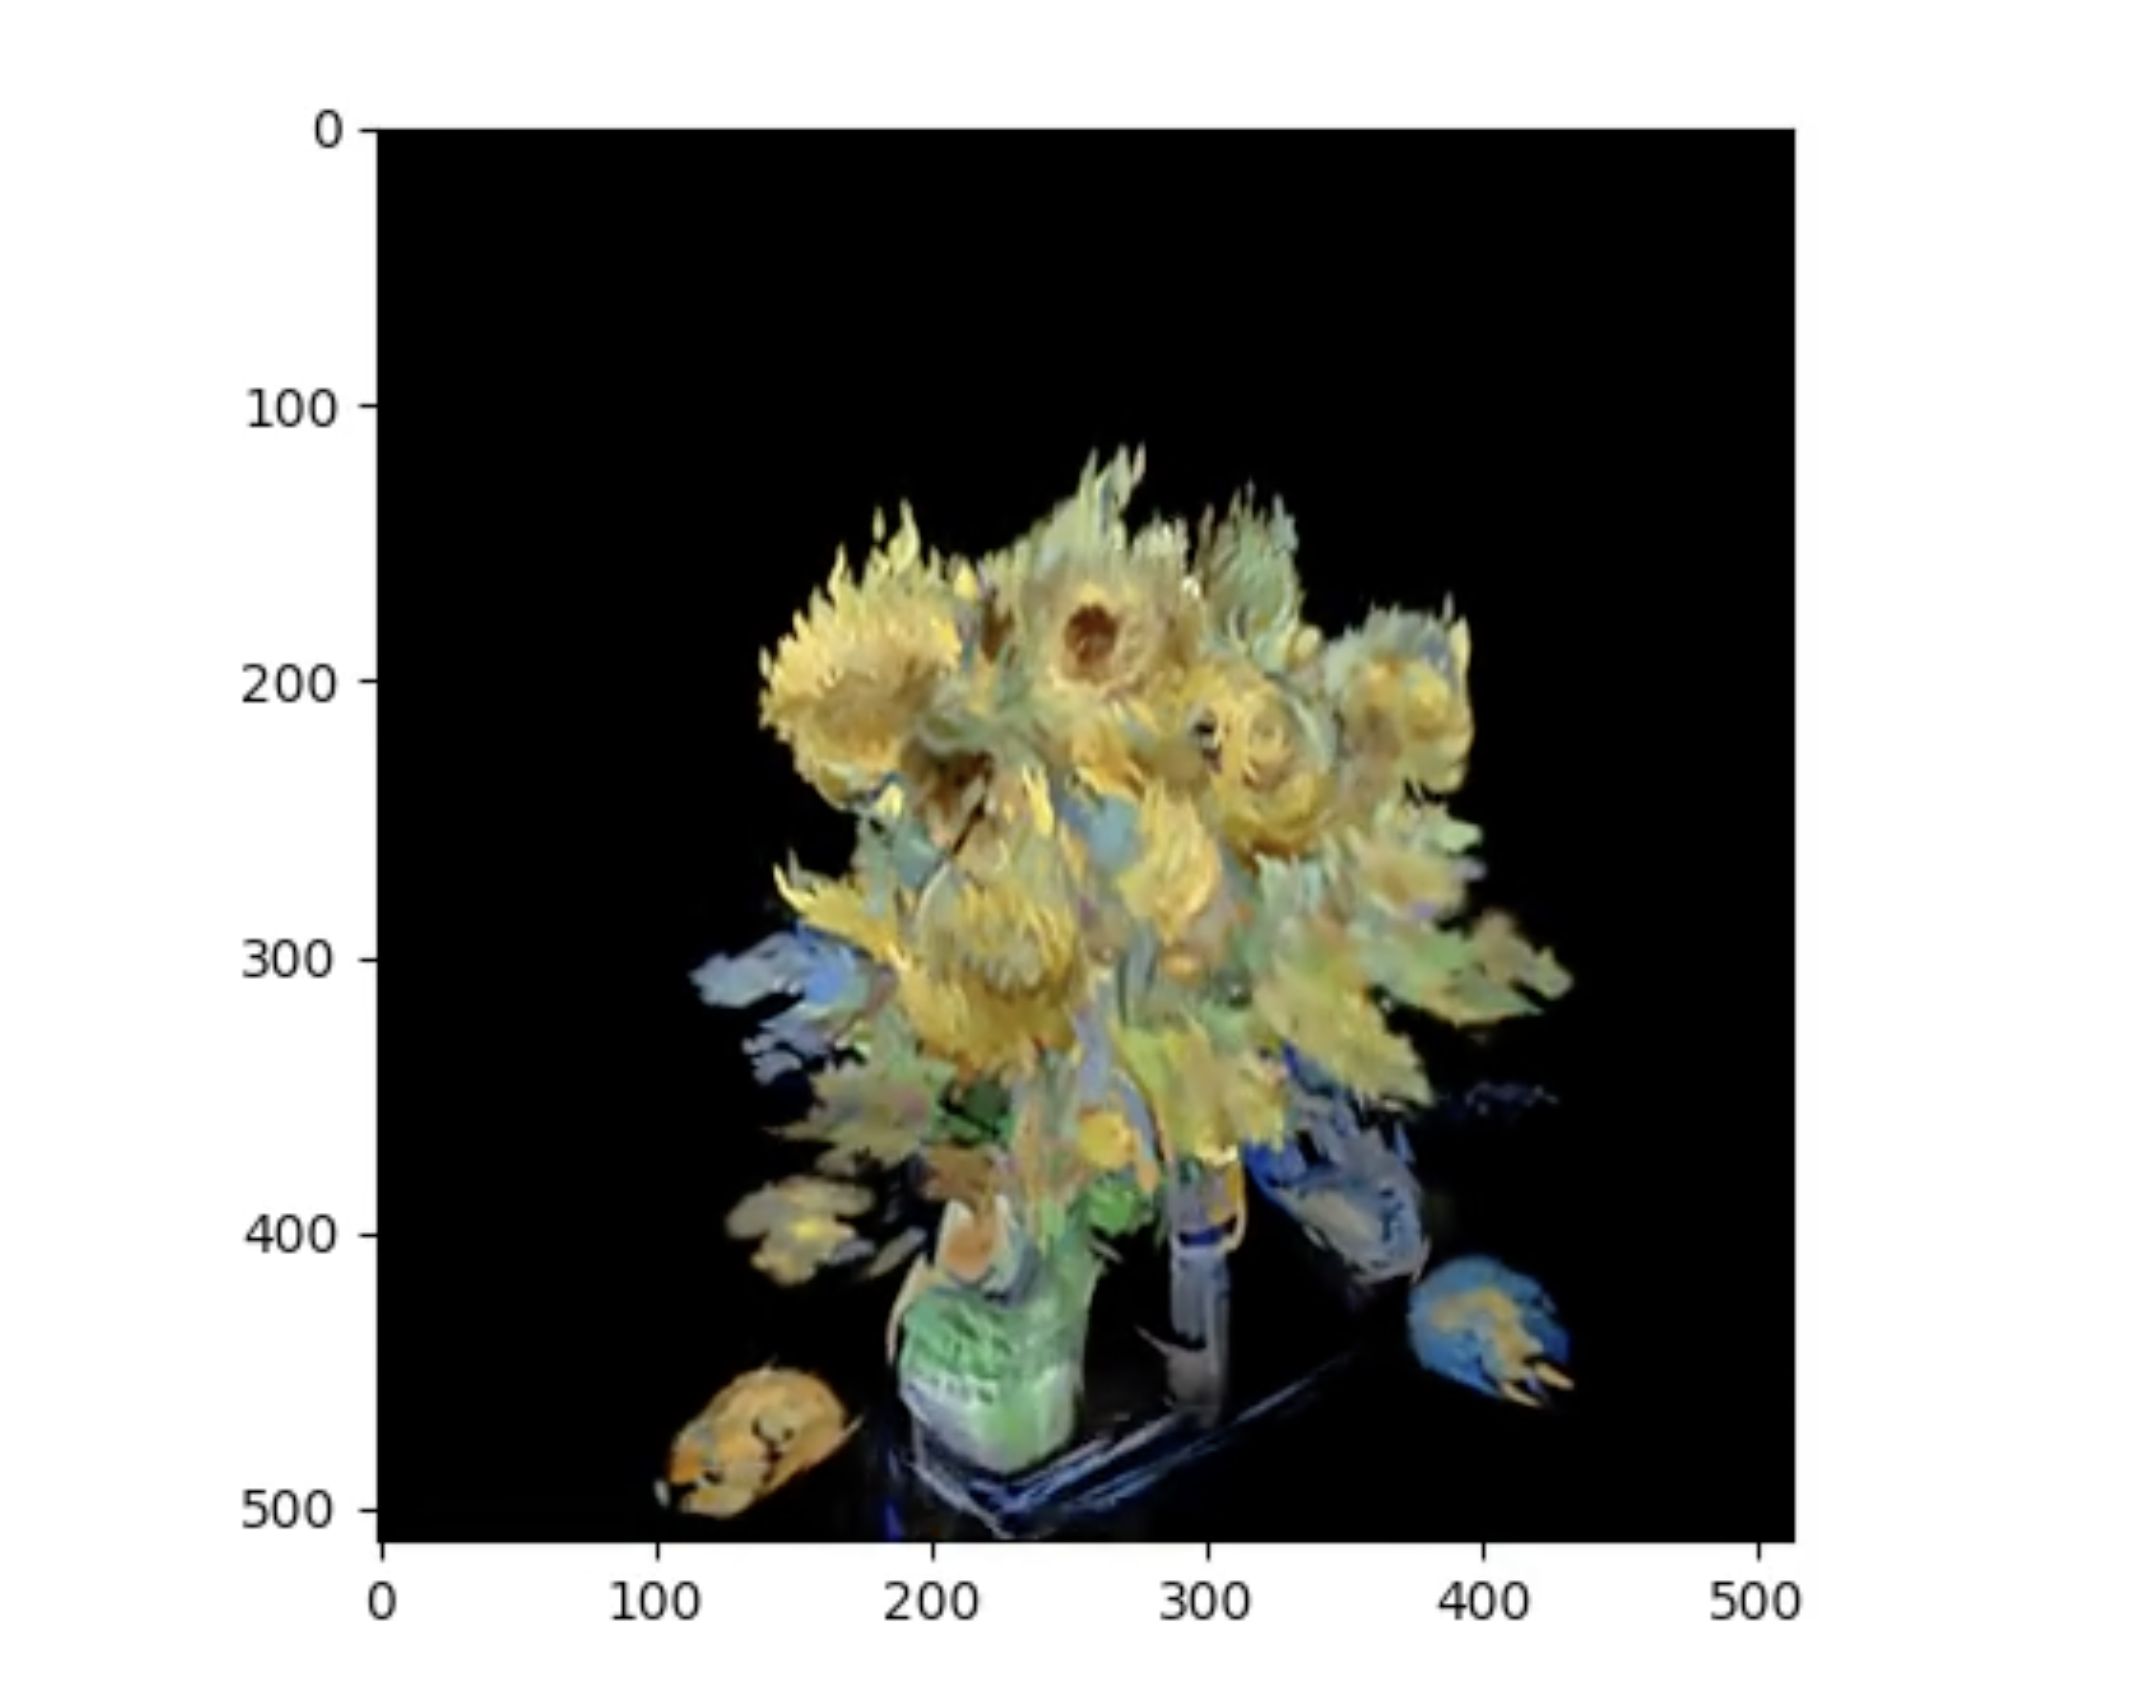
\includegraphics[width=0.6\textwidth]{sunflowers_3d_model.png}
    \caption{3D-модель подсолнухов Ван Гога, созданная с помощью текстово-управляемого гауссовского сплаттинга}
    \label{fig:sunflowers_3d}
\end{figure}

Полученная модель:

\begin{itemize}
    \item передаёт художественные особенности оригинальной сцены;
    \item поддерживает рендеринг с различных ракурсов;
    \item демонстрирует низкий уровень шума благодаря адаптивной плотности.
\end{itemize}

Таким образом, описанный подход подтверждает применимость гауссовского сплаттинга к задачам текстово-управляемой 3D-реконструкции, сочетая визуальную точность и эффективность дифференцируемого рендеринга.




\backmatter %% Здесь заканчивается нумерованная часть документа и начинаются ссылки и
            
\Conclusion

В ходе работы:

\begin{itemize}
    \item Изучены основы гауссовского сплаттинга (см. раздел~\ref{cha:analysis}).
    \item Реализована текстово-управляемая генерация 3D-сцен с использованием CLIP (см. раздел~\ref{cha:text_to_3d}).
    \item Построена 3D-модель подсолнухов Ван Гога (см. рис.~\ref{fig:sunflowers_3d}), подтверждающая корректность реализации.
\end{itemize}

\section*{Применение в робототехнике}

Разработанный метод может быть использован в следующих задачах:

\begin{itemize}
    \item \textbf{Навигация и SLAM} — построение детализированных 3D-карт и оптимизация маршрутов.
    \item \textbf{Обнаружение объектов} — текстово-управляемое распознавание и локализация в сцене.
    \item \textbf{Симуляция и обучение} — генерация реалистичных сцен для обучения агентов.
    \item \textbf{Обработка LiDAR-данных} — сглаживание, реконструкция и представление облаков точек в виде гауссиан.
\end{itemize}

\section*{Преимущества и ограничения}

\textbf{Преимущества:} высокая скорость рендеринга, поддержка динамических сцен, интеграция с языковыми моделями.\\
\textbf{Ограничения:} высокая вычислительная сложность, потребность в тонкой настройке гиперпараметров и производительном GPU.

\section*{Выводы}

Разработана и реализована система текстово-управляемой 3D-реконструкции на основе гауссовского сплаттинга. В перспективе возможны улучшения, направленные на:

\begin{itemize}
    \item оптимизацию под мобильные и встроенные устройства;
    \item интеграцию с физическими симуляторами;
    \item реализацию потоковой обработки в реальном времени.
\end{itemize}

\vspace{1em}
\section*{Репозиторий с исходными материалами}

Все исходные материалы, включая код, модели и примеры, находятся в открытом доступе на GitHub по адресу:
\begin{center}
  \href{https://github.com/SikioN/gaussian_splatting}{\texttt{gaussian\_splatting\_semantic}}
\end{center}
%% заключение


% % Список литературы при помощи BibTeX
% Юзать так:
%
% pdflatex rpz
% bibtex rpz
% pdflatex rpz

\bibliographystyle{ugost2008}
\bibliography{rpz}

\nocite{*}

%%% Local Variables: 
%%% mode: latex
%%% TeX-master: "rpz"
%%% End: 




\end{document}

%%% Local Variables:
%%% mode: latex
%%% TeX-master: t
%%% End:
